\section{Introduction}
Radio/(sub)-millimeter telescopes are powerful tools to study the universe at radio, sub-millimeter, and millimeter wavelengths.
These telescopes are designed to capture and detect electromagnetic radiation from space, which can provide valuable insights into a range of astronomical phenomena,
from the formation of stars and galaxies to the behavior of black holes.
One of the key components of a radio telescope is its reflective surface, which collects and focuses the incoming radiation.
Most radio/(sub)-mm telescopes have a large, parabolic dish-shaped primary mirror, reflecting incoming radiation onto a smaller, secondary mirror.
The secondary mirror then reflects the radiation onto a detector or receiver placed at the focal point, which records and processes the signals.\\

Radio/(sub)-mm telescopes detect and record photons over time, which are then processed to create a composite image or spectrum.
However, this process requires highly accurate pointing, as even slight errors in the telescope's orientation can significantly affect the resulting data quality.
Pointing errors, often referred to as pointing offsets, can be caused by various factors, including thermal deformation of the telescope components \cite{Dong2018},
gravitational deformation \cite{GravDeformation}, and other environmental factors like humidity and wind. As these factors may change over time, the offsets are also affected.
Most radio/(sub)-mm instruments do not have an imaging camera.
Hence, the correct positioning of the source within the resolution element (beam) and at the center of the field of view cannot be checked directly.
To achieve this accuracy, radio/(sub)-mm telescopes use pointing models, which take into account a range of factors that can contribute to the pointing error,
including weather conditions, telescope structure, and the target's position in the sky.\\

The Atacama Pathfinder EXperiment (APEX) telescope \footnote[1]{\href{http://www.apex-telescope.org/ns/}{Link to APEX website}}, located in the high-altitude Atacama Desert in Chile,
currently uses an effective analytical pointing model run in the background and recalibrated periodically through pointing measurement campaigns.
However, there is still a residual pointing offset whose origin is not completely understood.
This thesis aims to investigate two research questions.
First, we want to explore using machine learning to increase pointing accuracy based on observational data such as weather patterns and telescope pointing.
Secondly, we want to investigate a machine learning approach for developing pointing models for radio/(sub)-mm telescopes.
A machine learning approach would benefit larger radio/(sub)-mm telescopes like the future Atacama Large Aperture Submillimeter Telescope (AtLAST)
\footnote[2]{\href{https://www.atlast.uio.no/}{Link to AtLAST website}}.
AtLAST will have a $50$-meter diameter primary mirror and $12$-meter diameter subreflector. Hence, the subreflector will be as big as APEX's primary mirror.
Due to the size and complexity of AtLAST, it will be harder to develop an analytical model.
By developing a more advanced and reliable pointing model with machine learning,
this research can enhance the capabilities of current and future radio/(sub)-mm telescopes to advance our understanding of the universe.


\begin{figure}[H]
    \centering
    \begin{subfigure}[t]{0.49\textwidth}
        \centering
        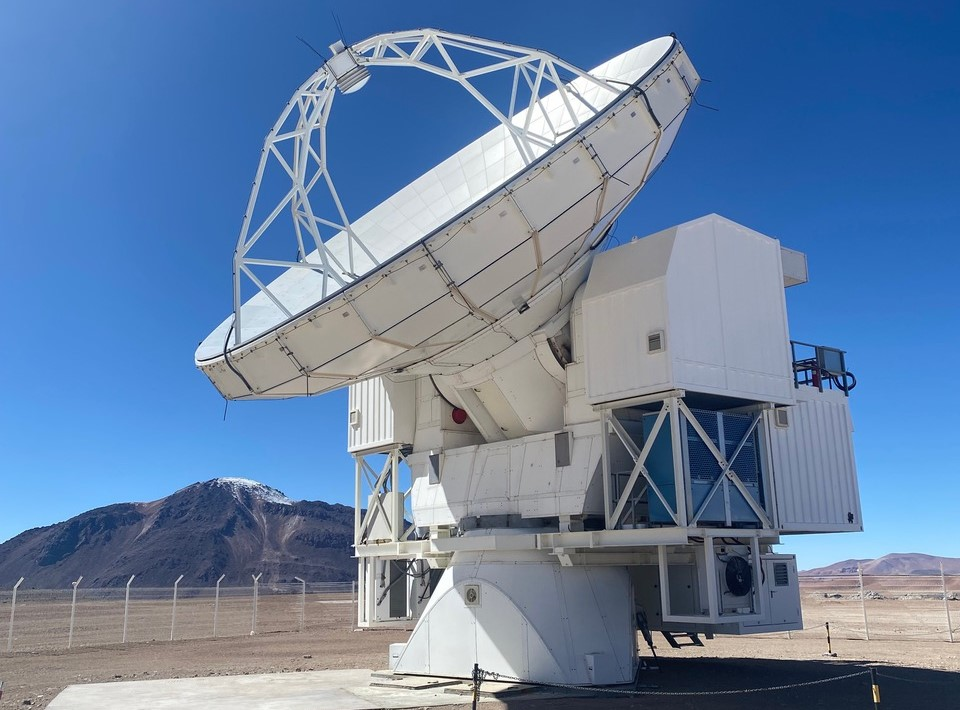
\includegraphics[width=\textwidth]{Astronomy/apex_primary_mirror_cropped.jpeg}
        \caption{Telescope structure. Credit: C. Cicone}
        \label{subfig:apex_primary}
    \end{subfigure}
    \hfill
    \begin{subfigure}[t]{0.49\textwidth}
       \centering
       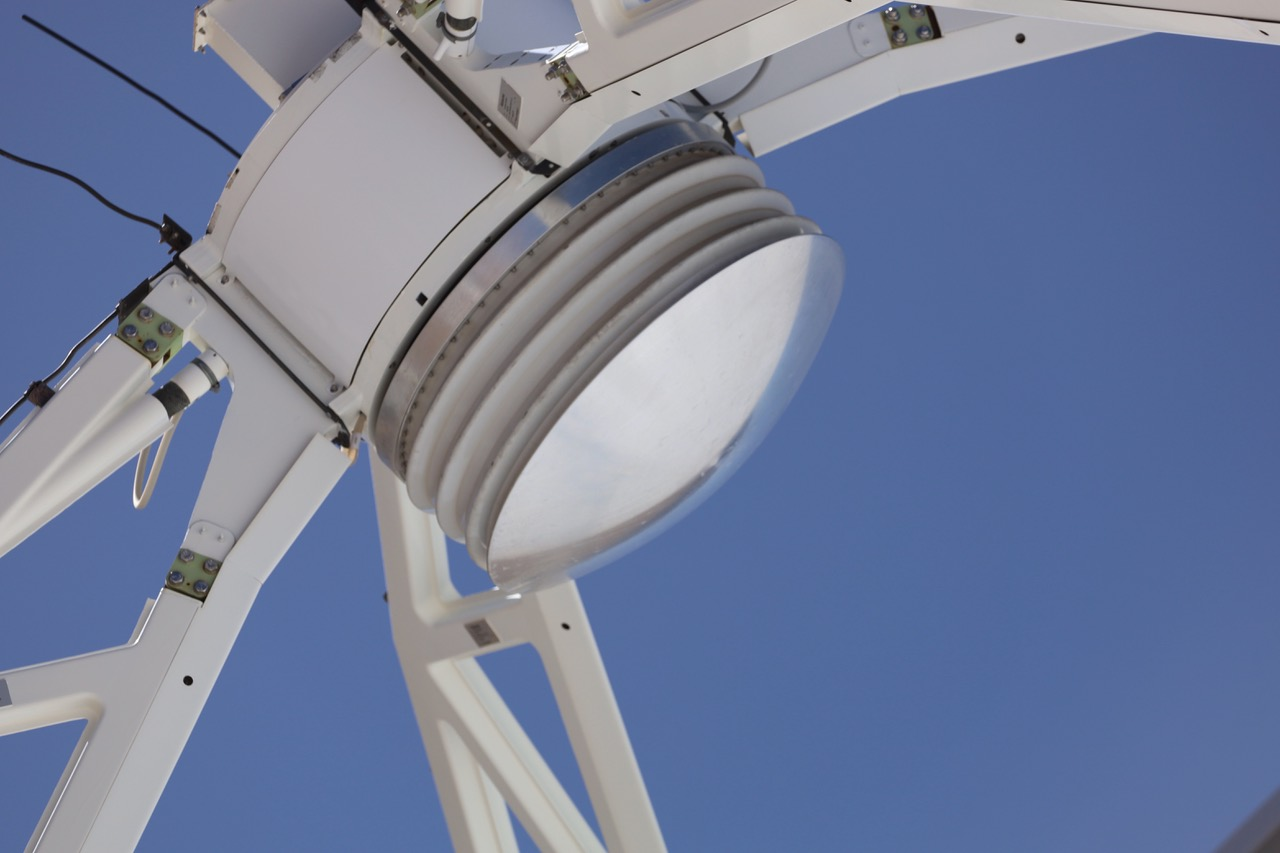
\includegraphics[width=\textwidth]{Astronomy/apex_subreflector.jpeg}
       \caption{Subreflector. Credit: P. Gallard}
       \label{subfig:apex_subref}
    \end{subfigure}
    \caption{Pictures of the APEX telescope}
    \label{fig:apex_images}
\end{figure}

